\documentclass[12pt]{article}
%%% ========== Package setup ==========
\usepackage{listings}   % Script listing package
\usepackage{wrapfig}    % Wrap Figure or table package
\usepackage{multicol}   % Multicolumn package
\usepackage{pdfpages}   % Include pdf files

%%% ========== Format setup ==========
%% Setup chinese words encoder
\usepackage{xeCJK}
\XeTeXlinebreaklocale "zh"
\XeTeXlinebreakskip = 0pt plus 1pt

%% More word fonts
\usepackage{fontspec}
\setmainfont{Times New Roman}
\renewcommand{\familydefault}{\rmdefault}
\setCJKmainfont{標楷體}

%% Chinese paragraph format
\usepackage{indentfirst}
\setlength{\parindent}{2em}

%% Page margin
\usepackage[a4paper, total={6in,8in}]{geometry}

%%% ========== Document ==========
\begin{document}
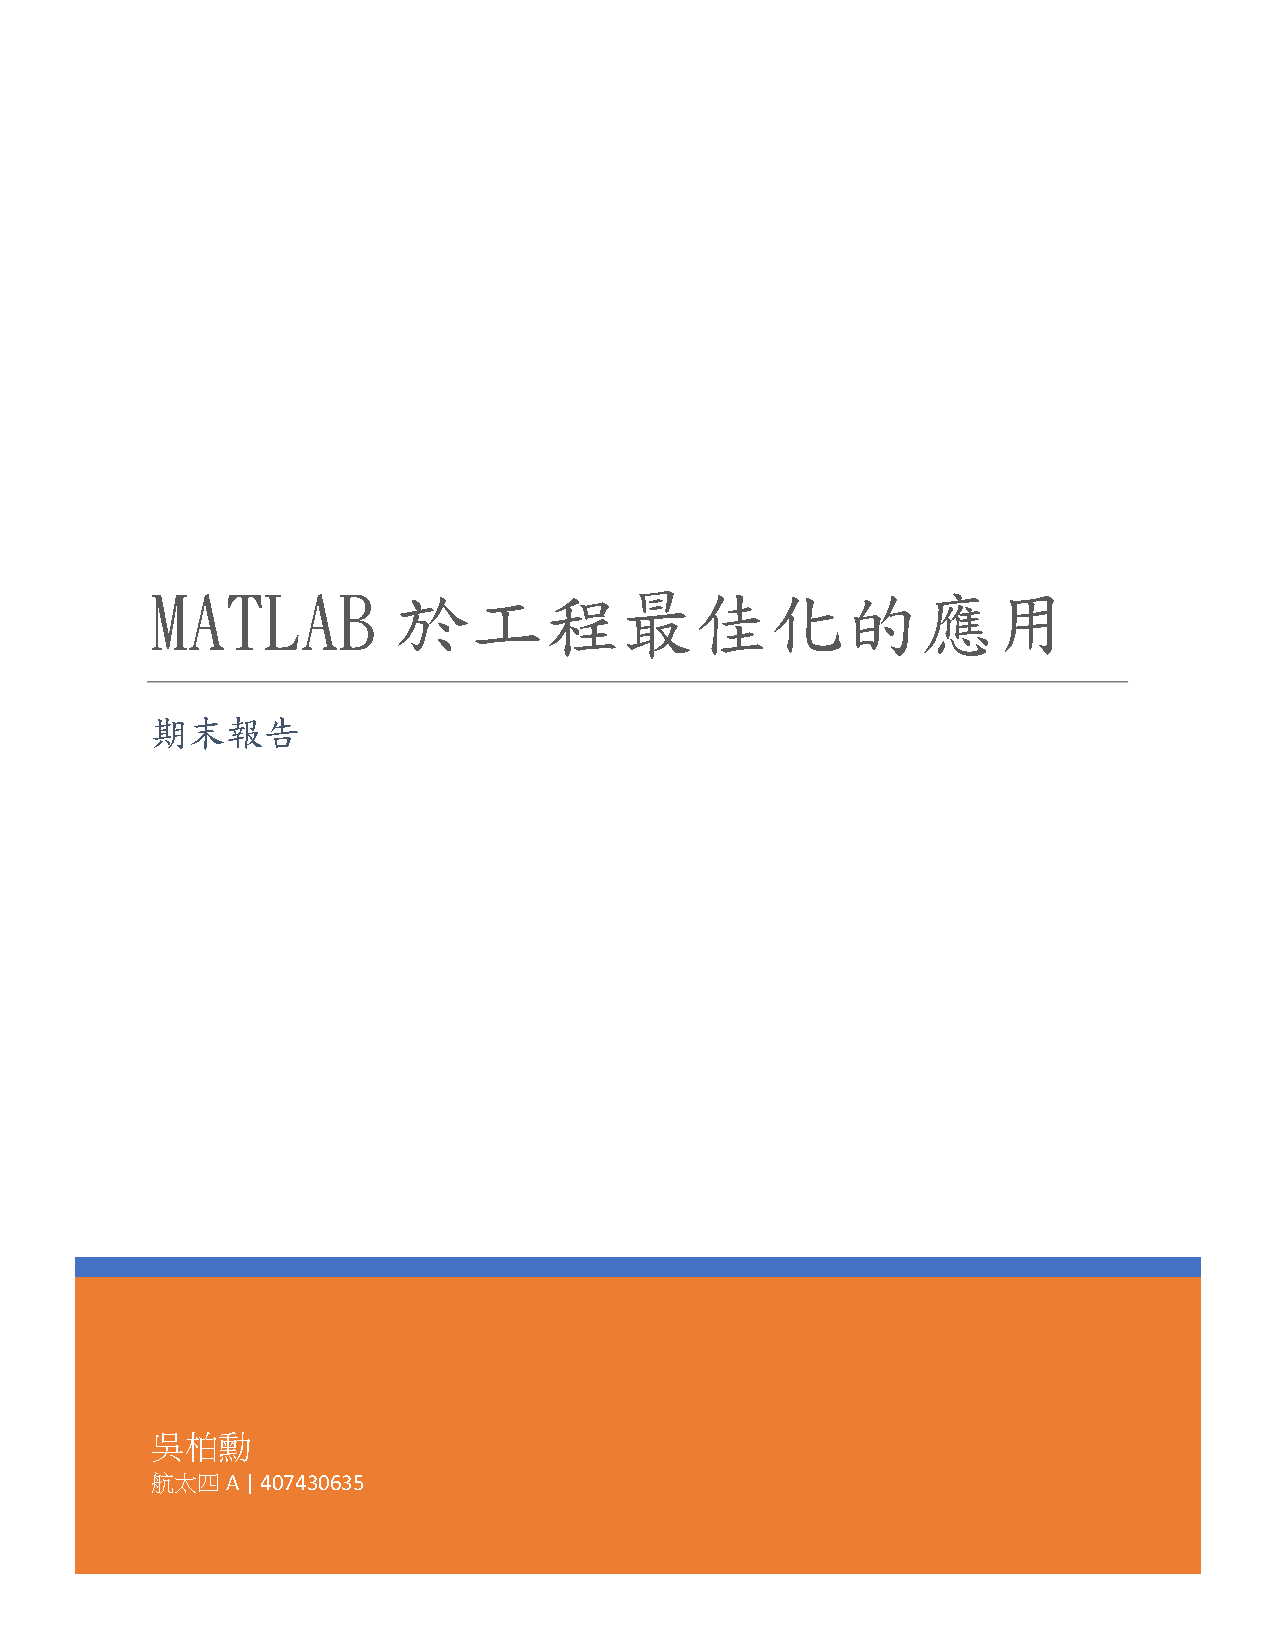
\includepdf[]{TitlePage.pdf}
\begin{verbatim}
clear;clc;close all
% Input and Target
P_2D = [1 1 1 1
        0 0 0 1
        0 0 0 1
        0 0 0 1
        1 1 1 1
        0 0 0 1
        0 0 0 1
        0 0 0 1
        1 1 1 1];
P = reshape(P_2D, 36, 1);
T = [0 0 1 1]';

% Initial W and b
W = randn(4, 36);
b = randn(4, 1);

% Call learn_p
[FW,Fb] = learn_p(P, T, W, b, 1, 0.001, 0)

% Check result
A = hardlim(FW*P+Fb)
\end{verbatim}

        \color{lightgray} \begin{verbatim}
===>Now running [Perceptron learning rule (learn_p)]. Please wait!

FW =

  Columns 1 through 7

   -0.4566   -0.6162    0.9460   -0.9936   -2.0914   -0.4901    1.1189
    0.5898    0.8805   -0.2842    0.8351   -1.0837    0.3370    1.3408
    1.4047    2.5430    1.2069   -0.7516   -0.2723    1.8425    2.5221
    0.4366    2.1817    0.2277   -1.1585   -0.9716   -1.2651    1.3129

  Columns 8 through 14

   -2.7440    1.5629    1.4182    0.4553   -0.0050    0.2123    0.6217
    0.4004   -0.7148    1.0770   -0.9131   -0.5766   -0.5279   -0.3543
   -0.5590   -0.0939    0.3709    0.4953    1.0540    0.3508    0.9536
    0.2408   -0.4161   -0.5535   -0.5244    0.6692   -1.1967   -0.1991

  Columns 15 through 21

   -0.6604   -0.3529    0.8011   -1.8192    1.6812    0.8484    1.2519
    0.7166    0.3811   -1.2928   -1.6924    0.2278    0.3102   -0.8024
    1.3312   -2.1975   -1.0246    0.6728   -0.5971    0.0629    1.0599
    0.0117   -0.2673   -0.9171    0.3697    0.6441    1.1588    0.4000

  Columns 22 through 28

    1.6597    1.3261   -1.0568   -0.0830    0.4295    0.8829   -0.7202
   -0.5036    0.7210    0.1021   -0.5644   -0.1232   -0.2684    0.5489
   -0.1338   -0.3199   -1.4535   -1.2814   -0.9545    0.4832    1.2338
    0.5907    0.7243   -1.2632   -0.2937    0.2311    0.0560   -0.3304

  Columns 29 through 35

   -0.1328    0.1133   -1.4621   -0.3482    0.1632   -0.1227   -0.3239
   -0.4997    0.1579    1.9282   -0.1130   -1.0460    0.8753    0.4931
    0.2876    0.7447    1.9097   -1.9595    0.4585    0.1304    0.6963
   -0.6176    0.9361   -0.0706    0.5106    0.8660    0.6597   -0.1060

  Column 36

   -0.0747
   -0.4760
   -0.3609
   -1.5387


Fb =

   -0.2187
   -0.3883
    0.7452
   -0.3869


A =

     0
     0
     1
     1

\end{verbatim} \color{black}


\subsection*{Check unlearned input patterns}

\begin{verbatim}
P_2D = [1 1 1 0
        0 0 1 1
        0 0 0 1
        0 0 0 1
        1 1 1 1
        0 0 0 1
        0 0 0 1
        0 0 1 1
        1 1 1 0];
P = reshape(P_2D, 36, 1);
A = hardlim(FW*P+Fb)
\end{verbatim}

        \color{lightgray} \begin{verbatim}
A =

     1
     1
     1
     1

\end{verbatim} \color{black}



\end{document}

